% Time-stamp: <Sunday 16 April 2023, Romain Lafarguette>
% Romain Lafarguette 2020, https://romainlafarguette.github.io/

%% ---------------------------------------------------------------------------
%% Preamble: Packages and Setup
%% ---------------------------------------------------------------------------
% Class 
\documentclass{beamer}

% Theme
\usetheme{Boadilla}
\usecolortheme{dolphin}
%\setbeamertemplate{headline}{} % Remove the top navigation bar

% Font and encoding
\usepackage[utf8]{inputenc} % Input font
\usepackage[T1]{fontenc} % Output font
\usepackage{lmodern} % Standard LateX font
\usefonttheme{serif} % Standard LateX font

% Maths 
\usepackage{amsfonts, amsmath, mathabx, bm, bbm} % Maths Fonts

% Graphics
\usepackage{graphicx} % Insert graphics
\usepackage{subfig} % Multiple figures in one graphic
\graphicspath{{/img}}

% Layout
\usepackage{changepage}

% Colors
\usepackage{xcolor}
\definecolor{imfblue}{RGB}{0,76,151} % Official IMF color
\setbeamercolor{title}{fg=imfblue}
\setbeamercolor{frametitle}{fg=imfblue}
\setbeamercolor{structure}{fg=imfblue}

% Tables
\usepackage{booktabs,rotating,multirow} % Tabular rules and other macros
%\usepackage{pdflscape,afterpage} % Landscape mode and afterpage
%\usepackage{threeparttable} % Split long tables
\usepackage[font=scriptsize,labelfont=scriptsize,labelfont={color=imfblue}]{caption}

% Import files
\usepackage{import}

% Appendix slides
\usepackage{appendixnumberbeamer} % Manage page numbers for appendix slides

% References
\usepackage{hyperref}

% A few macros: environments
\newenvironment{wideitemize}{\itemize\addtolength{\itemsep}{10pt}}{\enditemize}
\newenvironment{wideenumerate}{\enumerate\addtolength{\itemsep}{10pt}}{\endenumerate}

\newenvironment{extrawideitemize}{\itemize\addtolength{\itemsep}{30pt}}{\enditemize}
\newenvironment{extrawideenumerate}{\enumerate\addtolength{\itemsep}{30pt}}{\endenumerate}

% Remove navigation symbols and other superfluous elements
\setbeamertemplate{navigation symbols}{}
\beamertemplatenavigationsymbolsempty

%\setbeamertemplate{note page}[plain]
\hypersetup{pdfpagemode=UseNone} % don't show bookmarks on initial view
\setbeameroption{hide notes}

% Institute font
\setbeamerfont{institute}{size=\footnotesize}
\DeclareMathSizes{10}{9}{7}{5}

% Footnote without marker
\newcommand\blfootnote[1]{%
  \begingroup
  \renewcommand\thefootnote{}\footnote{#1}%
  \addtocounter{footnote}{-1}%
  \endgroup
}

%% ---------------------------------------------------------------------------
%% Title info
%% ---------------------------------------------------------------------------
\title[Introduction]{STI Course on FX Interventions \\ General Introduction}

\author[Lafarguette, Raboun, Chen]{Romain Lafarguette, Ph.D. \and Amine Raboun, Ph.D. \\ \and Zhuohui Chen}
\institute[IMF]{ADIA Quants \& IMF External Experts \& IMF MCM \blfootnote{\scriptsize{\emph{This training material is the property of the IMF, any reuse requires IMF permission}}} \\
\begin{center}{\href{https://romainlafarguette.github.io/}{\textcolor{imfblue}{www.romainlafarguette.github.io}} \hspace{0.3cm} \href{https://amineraboun.github.io/}{\textcolor{imfblue}{www.amineraboun.github.io}}} \end{center} \vspace{-0.5cm}} 

\date[STI, 17 April 2023]{\footnotesize Singapore Training Institute, 17 April 2023}

\titlegraphic{\vspace{-0.6cm}
    \begin{figure}
    \centering
    \subfloat{{
\includegraphics[width=2cm]{img/imf_logo}}}%
    \end{figure}}

  
%% ---------------------------------------------------------------------------
%% Title slide
%% ---------------------------------------------------------------------------
\begin{document}

\begin{frame}
\maketitle
\end{frame}


%% ---------------------------------------------------------------------------
%% Main Body
%% ---------------------------------------------------------------------------
\begin{frame}
  \frametitle{The Course Website}

Available via: \href{https://amineraboun.github.io/STI_FX_Intervention/docs/index.html}{\beamergotobutton{Course Website}}

%\makebox[\linewidth]{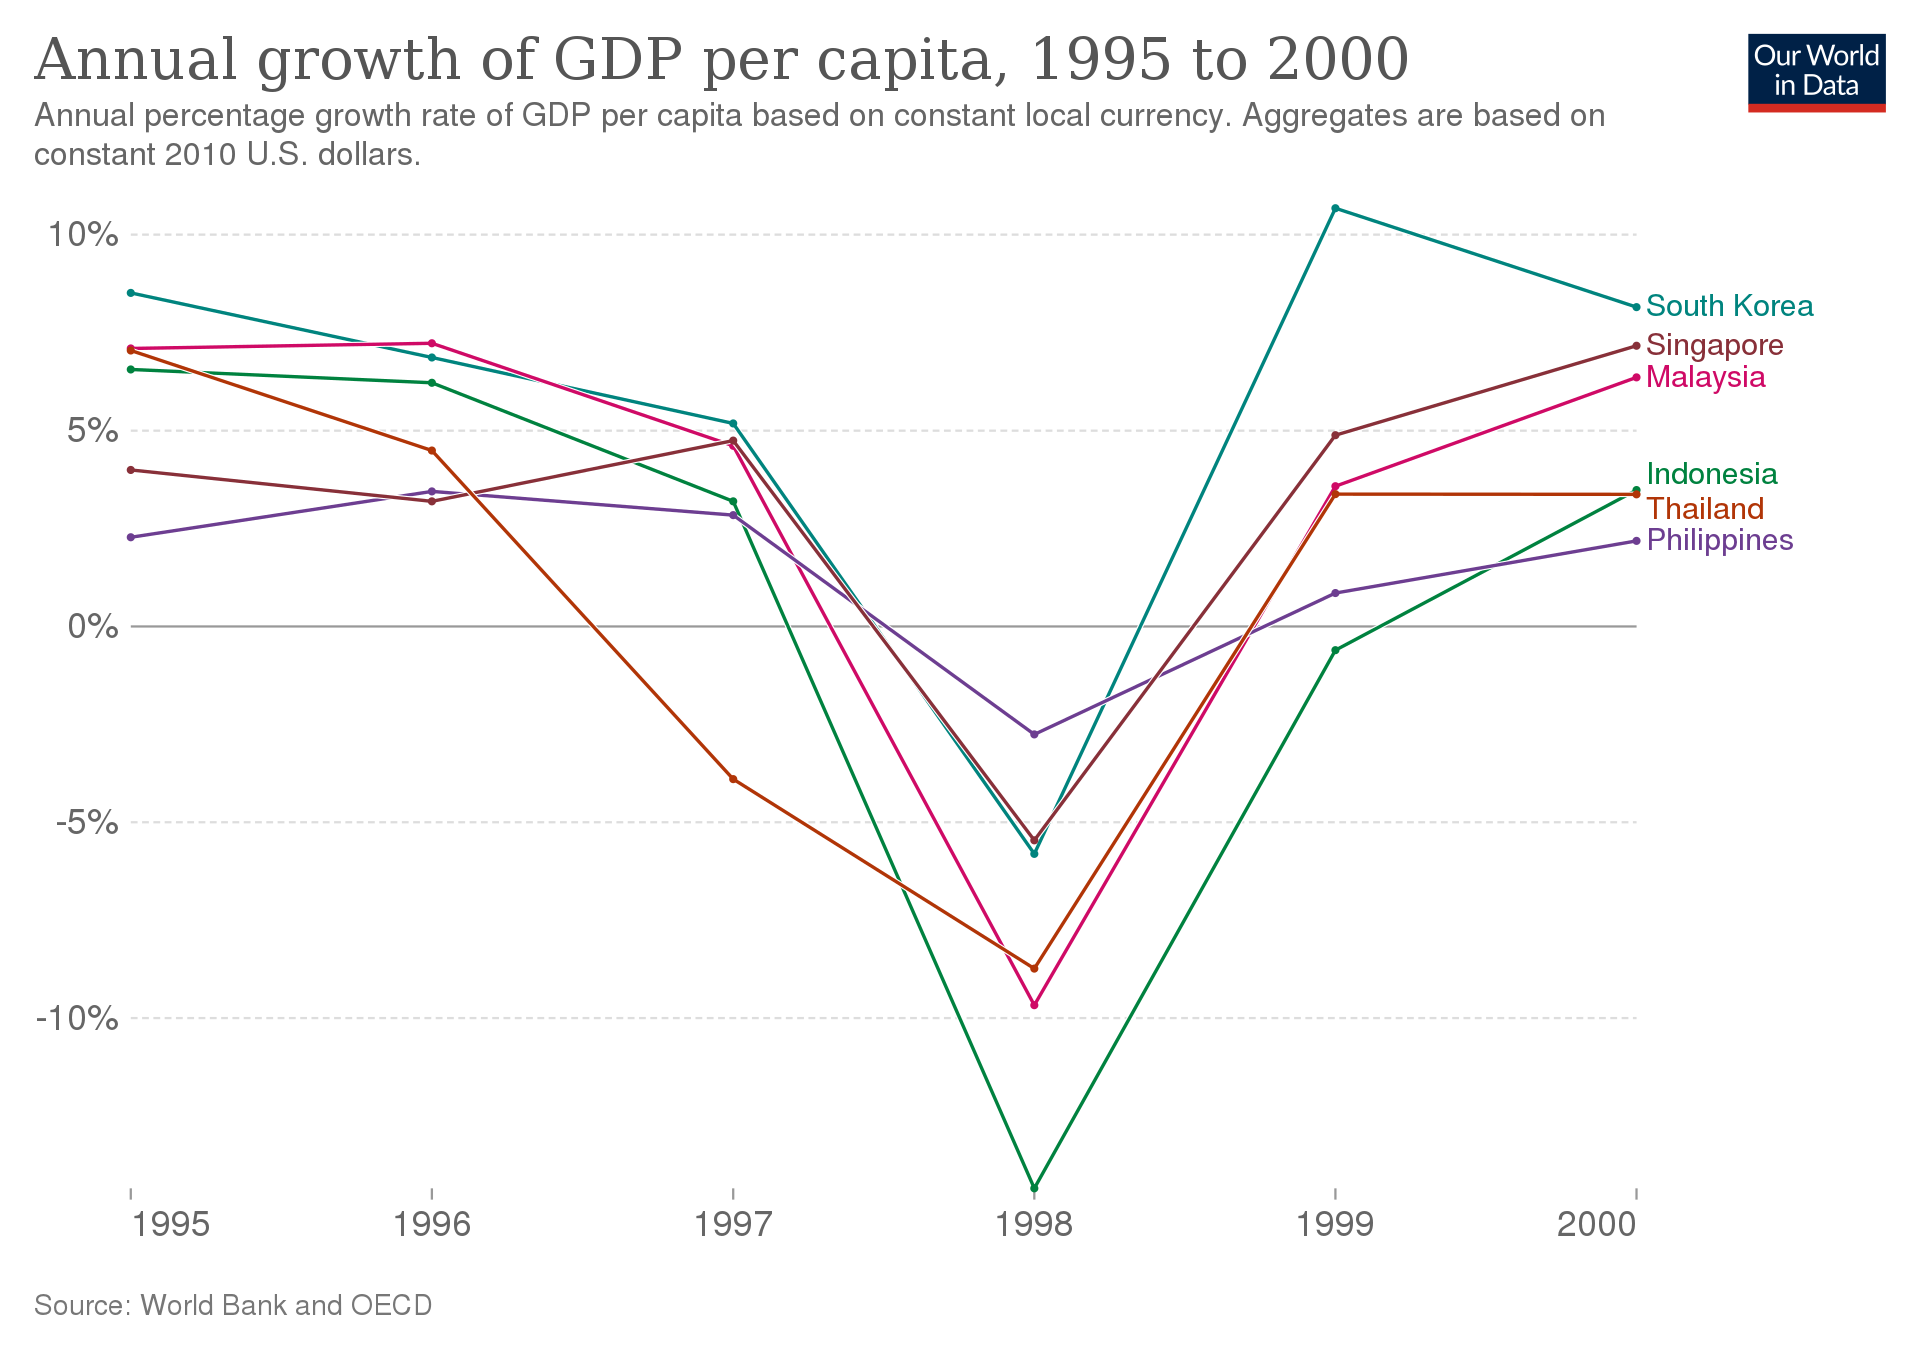
\includegraphics[width=0.75\paperwidth]{img/afc_gdp_crash.PNG}}
  
  
\end{frame}


\begin{frame}
  \frametitle{Overview}
  \begin{wideenumerate}
  \item Conceptual framework and academic literature on FX interventions 
    \begin{itemize}
    \item With a few country cases, illustrating the diversity of objectives and operational frameworks    
    \end{itemize}

  \item New risk-based IMF/MCM framework to time FX intervention rules from Lafarguette and Veyrune (2021)
    \begin{itemize}
    \item And using the new Python package developped by Lafarguette and Raboun (2023)
    \end{itemize}

  \item Training on volatility modeling and the econometrics of time series  
    
  \item Training on programming with Python
    
    
  \end{wideenumerate}

  
\end{frame}



\begin{frame}
  
\end{frame}



%% ---------------------------------------------------------------------------
%% End document
%% ---------------------------------------------------------------------------
\end{document}


%%% Local Variables:
%%% mode: latex
%%% TeX-master: t
%%% End:
